\documentclass[10pt]{beamer}
\usepackage[utf8]{inputenc}
\usepackage[T1]{fontenc}
\usepackage{lmodern}
\usepackage{microtype}
\usepackage[]{amsmath}
\usepackage{amssymb}
\usepackage{amsfonts}
\usepackage{appendixnumberbeamer}
\usepackage[czech]{babel}
\usepackage[]{hyperref}
\usepackage{booktabs}
\usepackage[]{graphicx}
\usepackage{media9}
\usepackage{siunitx}

\usepackage{listings}
\usepackage[]{color}
\definecolor{mygreen}{rgb}{0,0.6,0}
\definecolor{mygray}{rgb}{0.5,0.5,0.5}
\definecolor{mymauve}{rgb}{0.58,0,0.82}

\lstset{ 
  backgroundcolor=\color{white},   % choose the background color; you must add \usepackage{color} or \usepackage{xcolor}; should come as last argument
  basicstyle=\tiny,        % the size of the fonts that are used for the code
  breakatwhitespace=false,         % sets if automatic breaks should only happen at whitespace
  breaklines=true,                 % sets automatic line breaking
  captionpos=b,                    % sets the caption-position to bottom
  commentstyle=\color{mygreen},    % comment style
  deletekeywords={...},            % if you want to delete keywords from the given language
  escapeinside={\%*}{*)},          % if you want to add LaTeX within your code
  extendedchars=true,              % lets you use non-ASCII characters; for 8-bits encodings only, does not work with UTF-8
  frame=leftline,	                   % adds a frame around the code
  keepspaces=true,                 % keeps spaces in text, useful for keeping indentation of code (possibly needs columns=flexible)
  keywordstyle=\color{blue},       % keyword style
  language=Octave,                 % the language of the code
  morekeywords={*,...},            % if you want to add more keywords to the set
  numbers=left,                    % where to put the line-numbers; possible values are (none, left, right)
  numbersep=5pt,                   % how far the line-numbers are from the code
  numberstyle=\tiny\color{mygray}, % the style that is used for the line-numbers
  rulecolor=\color{black},         % if not set, the frame-color may be changed on line-breaks within not-black text (e.g. comments (green here))
  showspaces=false,                % show spaces everywhere adding particular underscores; it overrides 'showstringspaces'
  showstringspaces=false,          % underline spaces within strings only
  showtabs=false,                  % show tabs within strings adding particular underscores
  stepnumber=1,                    % the step between two line-numbers. If it's 1, each line will be numbered
  stringstyle=\color{mymauve},     % string literal style
  tabsize=2,	                   % sets default tabsize to 2 spaces
  title=\lstname                   % show the filename of files included with \lstinputlisting; also try caption instead of title
}
\usepackage[figurename=]{caption}
%\newcommand{\obr}[1]{Obr. převzat z \cite[#1]}

\usetheme[sectionpage=none, numbering=fraction, progressbar= head, block=fill]{metropolis}
\author{Michal Šesták}
\title{Python}
\subtitle{Matematické metody a modelování}
%\institute{}
%\institute{Fakulta jaderná a fyzikálně inženýrská, ČVUT v Praze\\[0.5em]
%Vedoucí práce: Ing. Iva Ambrožová, Ph. D.}
\date{9. 1. 2019}
\begin{document}
\small
%\footnotesize
%\scriptsize
\lstset{language=Python}
\maketitle

%\begin{frame}{Obsah}
    %\tableofcontents
%\end{frame}

\begin{frame}{Úvod}
    \begin{itemize}
        \item interpretovaný programovací jazyk, navržen v roce 1991, implementován v C (hlavní proud)
        \item dvě nekompatibilní verze: 2.x, 3.x (novější); vyvíjí se oba (2.x pomaleji); 2.x přestane být vyvíjen v roce 2020
        \item hybridní jazyk (objektově orientovaný a zároveň procedurální a funkcionální)
        \item dobře se čte a dá se velice rychle naučit
        \item ``Python a jeho mezery''
        \item pomalejší jazyk (cca 400x než C++), ale lepší ``development speed'' a méně kódu, je k dispozici zdarma
        \item silné balíčky, ideální pro zpracovávání dat, spousta triků
        \item široké použití (databáze, webové programování, aplikace (hlavně linuxové), hry, věda) 
    \end{itemize}
\end{frame}

\begin{frame}[fragile]{Charakteristiky}
    \begin{itemize}
        \item proměnná je pojmenovaným odkazem na objekt
\begin{lstlisting}[columns=fullflexible]
a = [1, 2]
b = a
del b[0]
a
[2]
\end{lstlisting}
\item Funkce se uchovává jako objekt
    \begin{lstlisting}[columns=flexible]
def funkce():
    print('Python')
f = funkce
p = [1, 2, 'test', f]
\end{lstlisting}
\item \dots
    \end{itemize}
\end{frame}

\begin{frame}[fragile]{Balíčky; indexování}
    \begin{itemize}
        \item \textbf{numpy, matplotlib, scipy}, pandas, math, random, datetime; sys, pdb, locale, time; SymPy (symbolic computation), seaborn, lmfit
\begin{lstlisting}[columns=fullflexible]
import numpy as np
import matplotlib.pyplot as plt
import pandas as pd
from scipy.optimize import curve_fit
\end{lstlisting}
\item Indexování:
    \begin{figure}
        \centering
        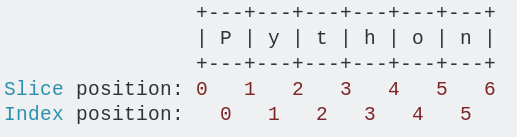
\includegraphics[width=.5\textwidth]{slicing.png}
    \end{figure}
    \end{itemize}
\end{frame}

\begin{frame}[fragile]{Slicing}
    \begin{itemize}
        \item základní
            \begin{lstlisting}[columns=flexible]
a[start:end] # items start through end-1
a[start:]    # items start through the rest of the array
a[:end]      # items from the beginning through end-1
a[:]         # a copy of the whole array

a[start:end:step] # start through not past end, by step

a[-1]    # last item in the array
a[-2:]   # last two items in the array
a[:-2]   # everything except the last two items

a[::-1]    # all items in the array, reversed
a[1::-1]   # the first two items, reversed
a[:-3:-1]  # the last two items, reversed
a[-3::-1]  # everything except the last two items, reversed
\end{lstlisting}
        \item numpy.array -> spousta triků
            \begin{lstlisting}[columns=flexible]
x = np.array([[ 0,  1,  2],
...           [ 3,  3,  5],
...           [ 6,  1,  8],
...           [ 9, 10, 11]])
x[:,0] #output je array([0, 3, 6, 9]), neboli prvni sloupec
x[x<5] #output je array([0, 1, 2, 3, 3, 1])
x[np.where(b<5)] #output je (array([0, 0, 0, 1, 1, 2]),array([0, 1, 2, 0, 1, 0]))
\end{lstlisting}
    \end{itemize}
\end{frame}

\begin{frame}[fragile]{For cyklus; příkazy in, enumerate, zip}
\begin{lstlisting}[columns=flexible]
my_list = ['apple', 'banana', 'grapes', 'pear']
for i in my_list:
    print(i)
# Output:
# apple
# banana
# grapes
# pear
for in np.arange(len(my_list)):
    print(i)
# Output:
# 0
# 1
# 2
# 3
for i, value in enumerate(my_list, 1): #druhy argument rika ze se indexuje od jednicky
    print(i, value)
# Output:
# 1 apple
# 2 banana
# 3 grapes
# 4 pear
alist = ['a1', 'a2', 'a3']
blist = ['b1', 'b2', 'b3']
for a, b in zip(alist, blist):
    print a, b
# Output
# a1 b1
# a2 b2
# a3 b3
\end{lstlisting}
        %\item List comprehension (pridej tam zip command) 
\end{frame}

\begin{frame}{Zpracovávání dat}
    \begin{itemize}
        \item \textbf{Numpy:} maticové počítání, ``náhrada matlabu'', rychlejší vektorové počítání, obsahuje matematické funkce (náhrada za balíček math)
            \begin{itemize}
                \item \emph{numpy.random}
                \item \emph{numpy.linalg} (lineární algebra)
            \end{itemize}
        \item \textbf{Scipy:} postaven na Numpy; \emph{optimization, linear algebra, integration, interpolation, special functions, FFT, signal and image processing, ODE solvers, statistics and other tasks common in science and engineering} 
        \item \textbf{Pandas:} nadstavba Numpy a matplotlib, rychlé zpracovávání dat a dělání grafů; I/O excel, html, latex \dots
        \item \textbf{IPython:} python prompt on steroids; it has completion, history, shell capabilities, and a lot more; případně \emph{Jupyter Notebook/Lab}
    \end{itemize}
    \begin{center}
        
\includegraphics[height=.2\textheight]{pandas.png}
    \end{center}
\end{frame}

\begin{frame}[fragile]{Fitování}
    \begin{itemize}
        \item np.polyfit
        \item scipy.optimize.curve\_fit
        \item lmfit
            \begin{lstlisting}[columns=flexible]
from numpy import loadtxt
from lmfit.models import GaussianModel, LorentzianModel, VoigtModel
import matplotlib.pyplot as plt
data = loadtxt('test_peak.dat')
x = data[:, 0]
y = data[:, 1]
mod = GaussianModel()
pars = mod.guess(y, x=x)
out = mod.fit(y, pars, x=x)
print(out.fit_report(min_correl=0.25))
parametry = dict(out.params)
A=out.params['amplitude'].value*out.params['sigma'].value*np.sqrt(2*np.pi) #plocha piku
out.plot_fit()
plt.show()
\end{lstlisting}
\vspace{-0.8cm}
\end{itemize}
\begin{columns}
    \centering
    \begin{column}{.65\textwidth}
        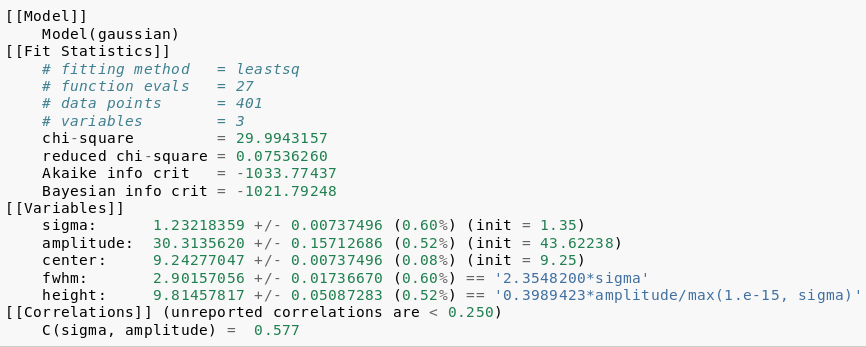
\includegraphics[width=\textwidth]{lmfit.png}
    \end{column}
    \begin{column}{.35\textwidth}
        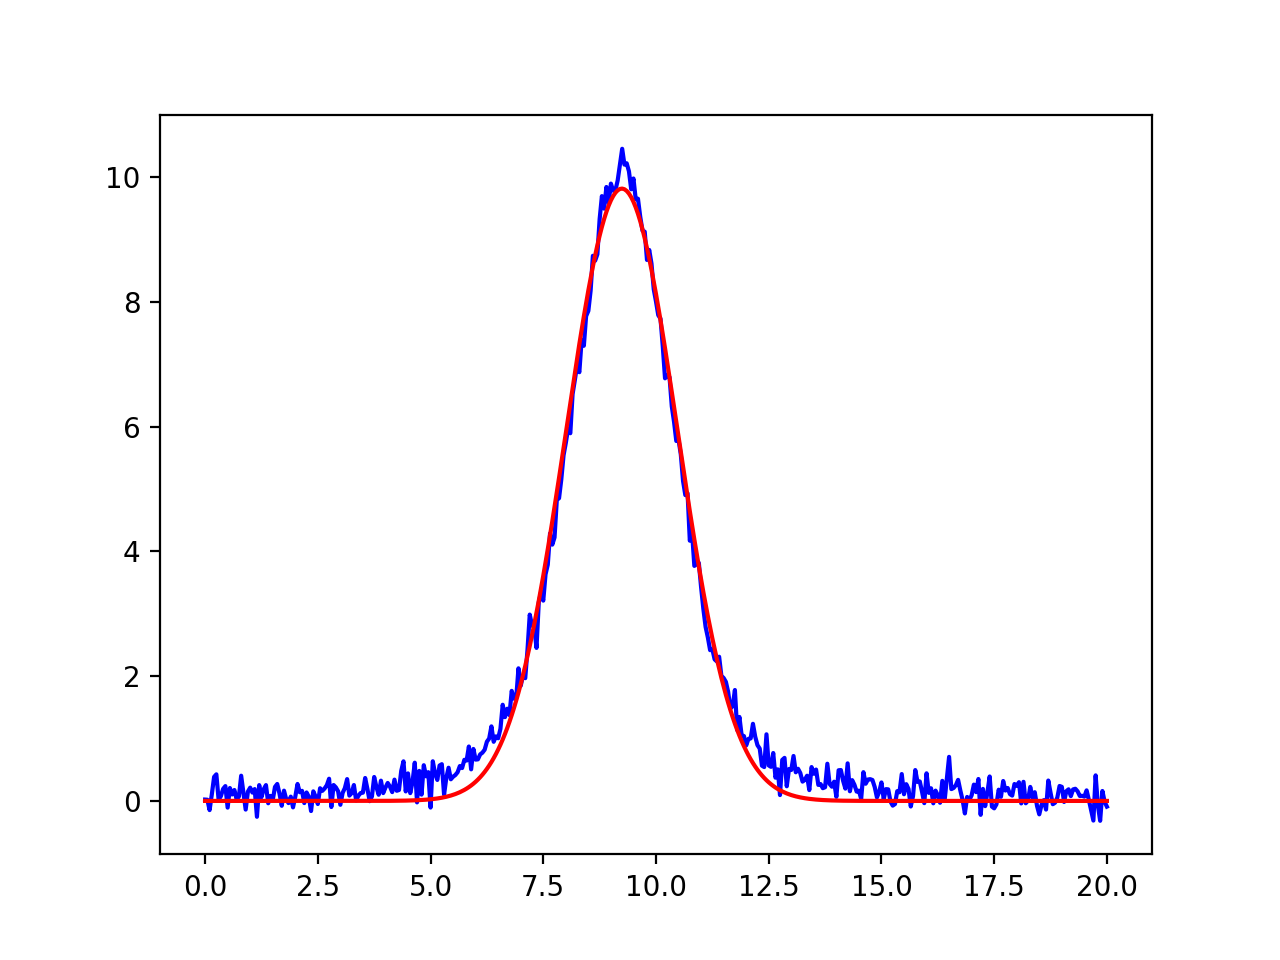
\includegraphics[width=\textwidth]{peak.png}
    \end{column}
\end{columns}
\end{frame}

\begin{frame}[fragile]{Příklad 1 -- Manganová lázeň}
V neutronové laboratoři byl pomocí metody manganové lázně charakterizován radionuklidový zdroj typu Am-Be. Ozařování bylo zahájeno 28. srpna 2017 v čase 9:48:43 a ukončeno 29. srpna 2017 v čase 10:48:38. Celková účinnost záchytu neutronů na nuklidu 55Mn je 0,38042 (relativní standardní nejistota údaje je 0,27 \%). Měření aktivity vzniklého radionuklidu 56Mn započalo 29. srpna 2017 v čase 11:28:00. Detekční účinnost sestavy se rovná 1,9113·10-3 (relativní standardní nejistota účinnosti je 0,39 \%). 
\begin{itemize}
    \item Z poskytnutého záznamu měření vypočítejte emisi neutronového zdroje.
\end{itemize}
\end{frame}

\begin{frame}[fragile]{Příklad 1 (2)}
\begin{lstlisting}[columns=flexible]
import matplotlib.pyplot as plt
import numpy as np
import datetime
from scipy.optimize import curve_fit

t0=datetime.datetime(2017,8,28,9,48,43) #pocatek ozarovani
t1=datetime.datetime(2017,8,29,10,48,38)#konec ozarovani
t2=datetime.datetime(2017,8,29,11,28,0) #zacatek mereni

prem_konst=np.log(2)/(2.5789*60*60) #[s^-1]
eps1=0.38042 #ucinnost zachytu
eps1_err=eps1*0.0027
eps2=1.9113e-3 #detekcni ucinnost
eps2_err=eps2*0.0039

data=np.loadtxt('Am-Be02.dat')

rozdil=int((t2-t1).total_seconds())
x=data[:,0]+rozdil
y=data[:,1]

def exponenciela(x,A0):
    return A0*np.exp(-prem_konst*x)

x_right=280
popt,pcov=curve_fit(exponenciela,x[:x_right],y[:x_right])
perr = np.sqrt(np.diag(pcov))
print(popt)
print(perr)
\end{lstlisting}
\end{frame}

\begin{frame}[fragile]{Příklad 1 (3)}
\begin{lstlisting}[columns=flexible]
#GRAF
fit='$A_{0}=$'+str(round(popt[0],0)).replace('.',',')+'$\pm$'+str(round(perr[0],0)).replace('.',',')
xp=np.linspace(x[0],x[x_right],num=x_right)
plt.semilogy(x,y,'x')
plt.plot(xp,exponenciela(xp,*popt),'r',label=fit)
plt.grid()
plt.xlabel('$t$ [s]')
plt.ylabel('$A$ [s$^{-1}$]')
plt.legend()
plt.show()

A0=popt[0]
A0_err=perr[0]

def vypocet_chyby(a,a0,eps,a0_err, eps_err):
    return a*np.sqrt((a0_err/a0)**2+(eps_err/eps)**2)

A=A0/eps2
A_err=vypocet_chyby(A,A0,eps2,A0_err,eps2_err)

S=A/eps1
S_err=vypocet_chyby(S,A,eps1,A_err,eps1_err)
print('Emise neutronového zdroje=('+str(round(S,-5))+' \pm '+str(round(S_err,-5))+') s^-1')
\end{lstlisting}
\end{frame}

\begin{frame}{Příklad 1 (výsledek)}
        \centering
        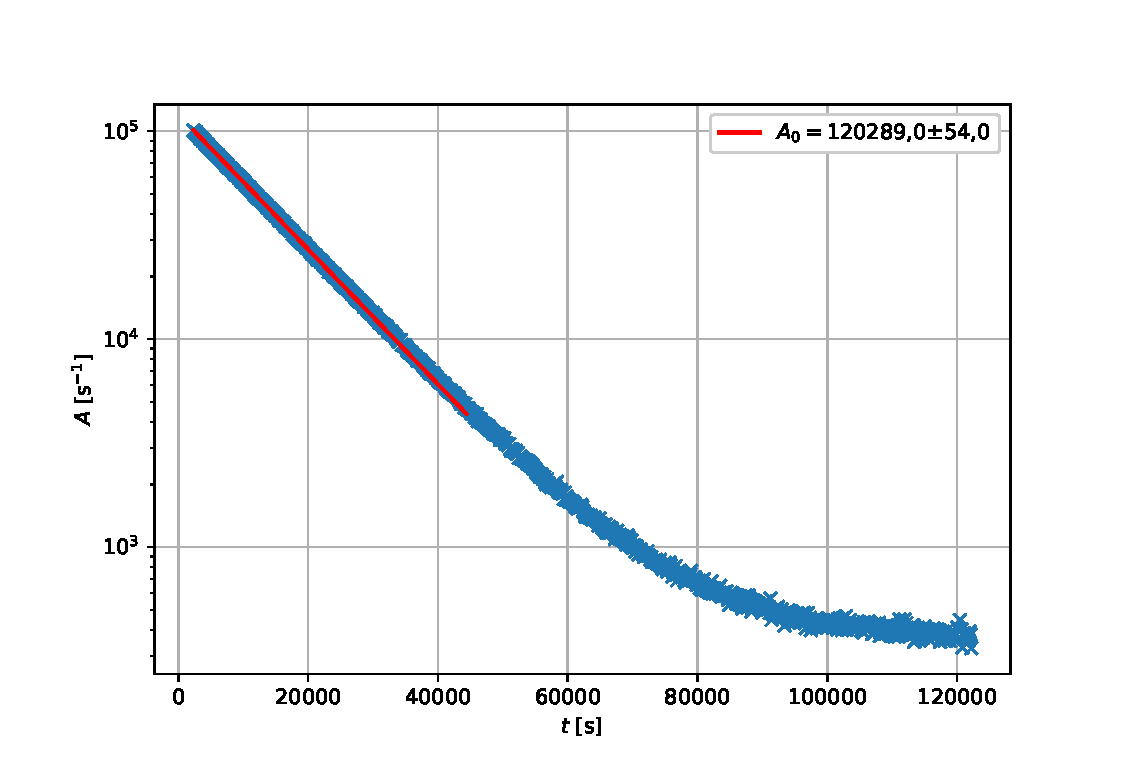
\includegraphics[height=.6\textwidth]{priklad1.eps}
\begin{equation}
    S=\SI[separate-uncertainty = true]{165,4(8)}{Ms^{-1}}
    \label{eq:priklad1}
\end{equation}
\end{frame}

\begin{frame}[fragile]{Příklad 2 -- Animace}
\begin{lstlisting}[columns=flexible]
import numpy as np
import scipy
import scipy.sparse.linalg
import matplotlib.pyplot as plt
import matplotlib.animation as animation
import time
import math
import pdb
import sys
#zde jsou definovany konstanty (polomer koule, pocatecni koncentrace vne koule, difuzni soucinitele, premenova konstanta

d=float(sys.argv[1]) # tloustka steny (0;0.1]
k_u=float(sys.argv[2]) #koeficient prestupu radonu na vnitrni okrajove podmínce
k_v=float(sys.argv[3]) #koeficient prestupu radonu na vnejsi okrajove podmince

def vypocet_CN(...,pp,D,c_u,c_v,tolerance=0.01,...)
    #Crank-Nicolsonova metoda pro numericky vypocet difuzni rovnice
\end{lstlisting}
\end{frame}

\begin{frame}[fragile]{Příklad 2 (2)}
\begin{lstlisting}[columns=flexible]
def animace(vysledek,c_u, c_v,tau,k,prostredi,interval=1,ulozit=False):
    '''
    Inputs:
        vysledek(array)
        c_u(array)
        c_v(float)
        tau(float)
    '''
    #zde se definuji objekty
    def animate(i):
        #zde se nastavuji objekty pro krok i
        return line, line_u, text_min,text_sek

    def init():
        #zde se nastavuji pocatecni hodnoty objektu
        return line, line_u, text_min, text_sek

    anim = animation.FuncAnimation(fig, animate, np.arange(0, k), init_func=init,
                                interval=interval, blit=True, repeat=False)
    if ulozit:
        anim.save('animace.mp4', fps=30, extra_args=['-vcodec', 'libx264'])
    plt.show()
\end{lstlisting}
\end{frame}

\begin{frame}[fragile]{Příklad 2 (3)}
\begin{lstlisting}[columns=flexible]
#nejake dalsi funkce vypocitavajici napr. nove pocatecni podminky

start=time.time()

#Prvni cyklus=NAPLNOVANI
k_t1,tau_t1,c_u_t1, vysledek_t1=vypocet_CN(T_t,pp,D_t,tolerance=0.01)
animace(vysledek_t1,c_u_t1,c0,tau_t1,k_t1,'tekute', interval=1)
#Urceni nove vnitrni okrajove podminky a pocatecni podminky
c_u_t0,pp_t=urcit_nove_pp(k_t1,c_u_t1,vysledek_t1)
#Druhy cyklus=VYPRAZDNOVANI
k_t2,tau_t2,c_u_t2, vysledek_t2=vypocet_CN(T_t,pp_t,D_t,c_u=c_u_t0,c_v=0,tolerance=0.01)
animace(vysledek_t2,c_u_t2,0,tau_t2,k_t2,'tekute', interval=1)
#Vypocet hledanych dob
t_t=k_t1*tau_t1+k_t2*tau_t2
print("\nDoba experimentu pro tekute prostredi: "+str(t_t)+" s; "+str(round(t_t/60,3))+" min; "+str(round(t_t/3600,2))+" hod")

stop=time.time()
print('\nSpotrebovany cas celkove: '+str(stop-start))
\end{lstlisting}
\end{frame}

\begin{frame}{Příklad 2 (výsledek)}
    \centering
 \includemedia[
    activate=onclick,
    width=0.7\textwidth
]{
\includegraphics{dots.png}}{animace1.swf}   
\end{frame}

% různá nastavení
%\metroset{sectionpage=simple,none}
%\begin{overlayarea}{\textwidth}{\textheight}\end{overlayarea}

\begin{frame}{Užitečné odkazy}
    \begin{itemize}
        \item \url{https://medium.freecodecamp.org/an-a-z-of-useful-python-tricks-b467524ee747}
        \item \url{https://en.wikipedia.org/wiki/Zen_of_Python}
        \item \url{https://docs.scipy.org/doc/numpy/user/numpy-for-matlab-users.html}
    \end{itemize}
\end{frame}

\begin{frame}{Reference}
    \begin{thebibliography}{Mm99}
        \bibitem{wiki} \url{https://cs.wikipedia.org/wiki/Python}
        \bibitem{slices} \url{https://stackoverflow.com/questions/509211/understanding-pythons-slice-notation}   
        \bibitem{cz} \url{https://python.cz/}
        \bibitem{slicing} \url{https://stackoverflow.com/questions/509211/understanding-pythons-slice-notation}
        \bibitem{comprehension} \url{}
    \end{thebibliography}
\end{frame}
%TO DO: grafy k prikladum, mp4 video,
\end{document}
